\documentclass[11pt]{article}
\usepackage{icmlko}
\begin{document}

\title{학습도 위를 뜨고 있었다 --- 대표 표본이 펀딩을 되살린다}
\author{월드모델 실험실}
\date{노트 381 · 2026년 8월 1일}
\maketitle

\begin{abstract}
노트 379가 펀딩 유보를 목록 상위 19\%에서 균일 표본으로 바꾸자 펀딩이
$+0.4195 \to +0.0866$ 으로 무너졌다. 그때 적어 둔 남은 것이 ``학습도 상위
19\% 다''였다. \textbf{같은 균일 표본의 2025년 이전 2,038건을 학습에만
더했다} --- 채점 집합은 529행 그대로라 노트 378 조항 ④(채점 집합이 같아야
한다)를 지킨다.

\textbf{펀딩 $+0.0866 \to +0.3112$, 판 $0.4057 \to 0.4355$.} 짝지은
부트스트랩 12회에서 판 $\mathbf{+0.0322}$ (SD 0.0102) $\cdot$
\textbf{12/12}, 펀딩 $+0.2260 \cdot$ 12/12 이고 $|t|>2.77$ 로 나빠진
도메인이 없다. \textbf{판이 직접 채택한다} --- 배포에 물어볼 필요도 없는,
최근 스무 노트에서 제일 큰 이득이다.

\textbf{그러니 노트 379의 무너짐은 절반이 모형 탓이 아니었다.} 옛 학습
320건의 후원자 중앙이 152명인데 균일 2,038건은 39명이다. 모형은 상위
구간만 보고 배운 뒤 전 구간에서 시험받고 있었다. 대표 표본으로 배우면
같은 모형이 같은 유보에서 3.6배를 낸다.

세 수를 나란히 놓으면 이번 수정의 정직한 값이 나온다: 옛 챔피언 0.4654 는
\emph{편향된 채점}과 \emph{편향된 학습}이 함께 만든 수이고, 채점만 고치면
0.4057, 학습까지 고치면 \textbf{0.4355} 다. \textbf{정직해진 대가는
$-0.0597$ 이 아니라 $-0.0299$ 였다.}
\end{abstract}

\section{쟀다}

\begin{figure}[t]
\centering
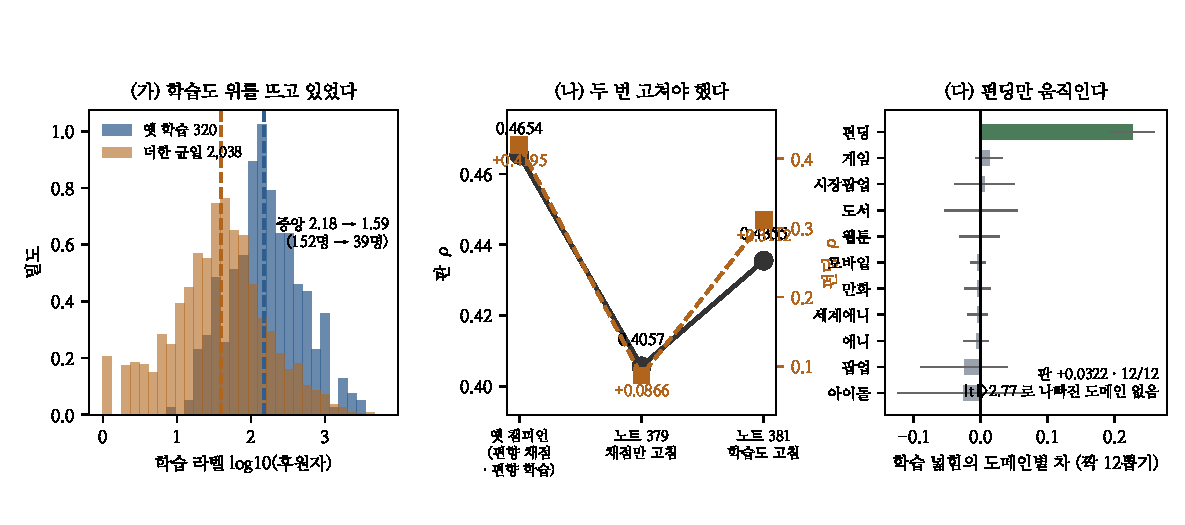
\includegraphics[width=\linewidth]{figs/fig381.pdf}
\caption{\textbf{(가)} 옛 학습 320건과 더한 균일 2,038건의 라벨 분포.
중앙이 $2.182 \to 1.591$(log10), 곧 후원자 152명 $\to$ 39명이다.
\textbf{(나)} 두 노트의 궤적 --- 채점만 고치면 판이 떨어지고 학습까지
고치면 대부분 돌아온다. \textbf{(다)} 학습 넓힘의 도메인별 차(짝 12뽑기,
막대는 짝 SD). 펀딩만 크게 움직이고 나머지 열은 0 근처다.}
\label{fig:main}
\end{figure}

\textbf{절차.} 노트 379가 채택한 챔피언(펀딩 849행 = 학습 320 + 유보 529)에
균일 표본의 \emph{2025년 이전} 2,038건을 더해 학습만 $320 \to 2{,}358$ 로
늘렸다. 유보 529행은 두 팔이 \textbf{같다} --- 노트 377이 찾고 노트 378이
조항으로 넣은 ``채점 집합이 다르면 잴 수 없음''을 피하기 위해서다.
펀딩 \texttt{trend\_*} 는 노트 379가 이미 막아 뒀으므로 새 학습 행이 배치
표시자를 새로 만들지 않는다.

\begin{center}
\begin{tabular}{lrrr}
\hline
 & 판 & 펀딩 & 펀딩 학습 \\
\hline
A 챔피언 & 0.4057 & $+0.0866$ & 320 \\
B 균일 학습 더함 & \textbf{0.4355} & $\mathbf{+0.3112}$ & 2,358 \\
\hline
짝 12뽑기 차 & $+0.0322$ (SD 0.0102) & $+0.2260$ & \\
부호 & \textbf{12/12} & \textbf{12/12} & \\
\hline
\end{tabular}
\end{center}

판 부호가 12/12 라 노트 378 조항 ①로 \textbf{판이 직접 정한다.} 조항 ②의
``어느 도메인도 $|t|>2.77$ 로 안 나빠진다''도 만족한다 --- 제일 나쁜 것이
아이돌 $-0.0261$(SD 0.0977, $t=-0.27$)과 팝업 $-0.0245$(SD 0.0651,
$t=-0.38$)이다.

\section{읽는 법}

\textbf{모형이 못 하던 게 아니라 안 배운 것이었다.} 노트 379는 균일 유보
449행에서 예측이 죽지 않았다는 것을 확인했다(서로 다른 예측 434개) ---
모형은 잴 수 있었고 다만 틀렸다. 왜 틀렸나에 대한 답이 이것이다: 학습
라벨 중앙이 152명인데 유보 중앙은 29명이라, 모형이 배운 구간과 시험받는
구간이 달랐다.

\textbf{그리고 이것은 판에서만 보이는 이득이 아니다.} 펀딩 하나가
$+0.2260$ 을 내고 나머지 열 도메인의 차가 전부 $|0.013|$ 안이다 --- 노트
258이 경고한 ``전용 축을 더하면 제일 큰 도메인이 내려간다''가 여기서는
안 일어난다. 학습 행을 더하는 것은 열을 더하는 것과 다르다.

\textbf{세 수를 같이 적는다.}

\begin{center}
\begin{tabular}{lrl}
\hline
 & 판 & \\
\hline
옛 챔피언 & 0.4654 & 편향된 채점 · 편향된 학습 \\
노트 379 & 0.4057 & 채점만 고침 \\
노트 381 & \textbf{0.4355} & 학습까지 고침 \\
\hline
\end{tabular}
\end{center}

노트 379를 혼자 읽으면 ``정직해지니 판이 $-0.0597$''인데, 그것은
\textbf{절반만 고친 상태의 수}였다. 정직한 값은 $-0.0299$ 다. 노트 379가
``점수가 내려가는 건 안 넣을 이유가 아니다''라고 쓴 것은 그대로 옳지만,
\textbf{내려간 김에 왜 내려갔는지 끝까지 갈랐어야 했고 이번에 갈랐다.}

\section{이것이 다른 도메인에도 있는가}

거의 확실히 있다. 노트 375가 아홉 도메인을 절단 · 구역 편향 · 열림으로
분류했고, 펀딩은 그중 하나였을 뿐이다. \textbf{다만 지금은 펀딩에만 대표
표본이 있다} --- 다른 도메인에서 같은 것을 하려면 같은 균일 수집이 필요하고,
그것이 지금 제일 값이 큰 수집이다.

\textbf{주의 하나.} 펀딩 학습이 320에서 2,358로 늘어 이제 판에서 제일 큰
학습 도메인이다(세계애니 2,648 다음). 이것이 다른 도메인의 계수를 얼마나
끌어당기는지는 이번 12뽑기에서 안 보이지만(나머지 열이 $|0.013|$ 안),
같은 일을 두세 도메인에 더 하면 그때는 봐야 한다 --- 노트 246\,--\,250의
공유 계수 이야기가 그 자리다.

\section{남은 것}

\begin{center}
\begin{tabular}{lll}
\hline
항목 & 왜 값이 큰가 & 어떻게 \\
\hline
다른 도메인 균일 수집 & 이번 이득이 반복될 수 있는 유일한 길 & 노트 375 분류에서 구역 편향부터 \\
펀딩 트렌드 2,487 & 막은 열 셋을 되살린다 & 새 행 트렌드 수집 \\
학습 크기 대 대표성 & 2,038행 중 무엇이 일했나 & 균일 320행만 넣어 견준다 \\
팝업 실측 41행 & 배포가 65행이다 & 수집 \\
\hline
\end{tabular}
\end{center}

\end{document}
